\chapter{基于变分推断的高阶方法}
\label{cha:vi}

本章节在章节~\ref{cha:dep-crf}和~\ref{cha:con-crf}提出的高阶TreeCRF句法分析器的基础上,提出了一个近似的MFVI算法来代替精确推断的高阶方法.
因为建模简单性能优异,基于图的句法分析方法一直以来是目前最流行的句法分析方法之一.
而其中的高阶TreeCRF方法由于融入了包含更多变量交互的子树特征,并且具备估计概率分布的优势,一直以来都是一个有吸引力的研究方向.
然而,由于Inside-Outside推断算法高复杂问题,限制了高阶TreeCRF的应用.
在本章中,我们提出利用基于MFVI的近似算法来代替精确推断的高阶TreeCRF,从而显著降低了推断算法的复杂度.
与其他近似方法相比,MFVI方法具备了方便地获取树/子树概率的优势.
我们在依存句法和成分句法的中英文常见的5个基准数据集上做了实验,并对比了加入BERT之后的效果.
结果表明,MFVI方法不仅从准确率上相匹敌,并且训练和测试的速度要远远快于章节~\ref{cha:dep-crf}和~\ref{cha:con-crf}里的高阶TreeCRF方法.

\section{引言}\label{sec:vi-intro}
近年来句法分析领域有了长足的进步.
研究者针对句法分析任务提出了一系列的方法 \citep{dozat-etal-2017-biaffine,gomez-rodriguez-vilares-2018-constituent,ji-etal-2019-graph,zhang-etal-2020-fast,wei-etal-2020-span},将英语基准数据集宾州树库(Penn Treebank, PTB)的准确率刷新到了很高的水平.

作为代表性的方法之一,基于图的方法选择将一棵句法树分解为多个部分,然后分别打分,组成树的分值,并训练模型使得能够找到分值最大的句法树.
相比基于转移的方法,基于图的方法建模简单,并且通常不会陷入局部最优,因此依存句法和成分句法中很多工作都遵循了这个范式 \citep{mcdonald-etal-2005-non,mcdonald-etal-2005-online,taskar-etal-2004-max}.
最简单的一阶基于图的方法让树中的每个变量都互相独立,例如要求依存树的每条弧均互相独立(称为弧分解假设)或者成分树的每个区块互相独立.
后来,有研究者提出放宽一阶假设,考虑包含更多子结构的交互的高阶特征,发现显著提升了句法分析器的性能 \citep{mcdonald-pereira-2006-online,koo-collins-2010-efficient,ma-zhao-2012-fourth}.
最近,有很多文献在神经网络模型中引入了二阶子树特征 \citep{chen-manning-2014-fast,ma-hovy-2017-neural,pei-etal-2015-effective}.
其中,\citet{ji-etal-2019-graph}在当前最流行的基于一阶局部训练目标的Biaffine Parser的基础上,考虑了祖孙、兄弟等二阶子树,并利用多层GAT来编码.
这些工作证明了高阶方法在基于神经网络的模型中是有益的.

尽管有很好的性能,现有的基于图的高阶方法中存在着一些固有问题限制了其应用.
一方面,为了找到最优的句法树,高阶方法需要设计高复杂度的动态规划算法来求解,当引入更多复杂的子树特征时,我们往往无法得到一个可精确推断的算法,尽管我们在章节~\ref{cha:dep-crf}和章节~\ref{cha:con-crf}展示了如何通过批次化等方法加速,但是推断算法的复杂度仍然带来了不可忽视的时间开销.
另一方面,由于效率原因,现有的工作通常采用Max Margin方法 \citep{mcdonald-pereira-2006-online}或者局部目标 \citep{ji-etal-2019-graph}来训练,而非需要全局归一化的TreeCRF.
而对于句法分析社区而言,一个重要的目的是概率分布推断\footnote{我们提到的句法分析中的概率分布推断通常指的是两个方面:1)MAP Inference,即获取概率最大的句法树;2)Marginal Inference,即得到每个变量的边缘概率.}.
无论是为了获得性能更高的分析器,还是作为特征应用到下游任务中 \citep{zhang-etal-2019-syntax,zhang-etal-2020-syntax},树和子树的后验/边缘概率都是重要的.

针对这些问题,在本章中,我们提出基于平均场变分推断的近似方法到高阶依存句法和成分句法分析模型中(Mean Field Variational Inference, MFVI).
对于不可精确推断问题采用近似方法一直以来都在图像分割、句法分析等领域有广泛的应用 \citep{krahenbuhl-etal-2011-efficient,wang-etal-2019-second,martins-etal-2011-dual}.
其中作为与我们最相关的工作,\citet{smith-eisner-2008-dependency,gormley-etal-2015-approximation}提出应用循环置信传播算法融入大量的全局因子,如约束全局树的\textsc{Tree}、双变量子树的\textsc{Sib}和\textsc{Grd}等来帮助依存句法模型,\citet{fonseca-martins-2020-revisiting}则应用了基于对偶分解的$AD^3$算法处理Siblings/Grandparents等特征.
我们选择MFVI,理由有两个:1)为了与前面章节保持一致,我们采用了不超过两个变量的二阶子树特征,在这个场景下,相比于循环置信传播,MFVI的收敛更快,复杂度更低;2)与对偶分解相比,MFVI可以方便地得到边缘概率,方便我们进行MBR解码.

本章中,针对依存解析和成分解析两种任务的特性,我们分别为他们设计了不同的因子图和MFVI更新算法.
依存句法中,由于每个位置都只有一个头,因此参考\citet{wang-tu-2020-second},我们的MFVI算法设计中引入了头选择的结构约束,让每个位置取值在所有可能的头上归一化.
成分句法中,我们参考\citet{naradowsky-etal-2012-grammarless,wang-etal-2019-second,smith-eisner-2008-dependency},让句法树的每个组块对应变量的取值为0-1.
我们发现近似算法在获取了和精确推断的高阶模型相接近的准确率的同时,解析速度大大提高.

总体而言,我们在本章节的工作如下:
\begin{itemize}
	\item 我们提出在句法分析任务上应用引入二阶特征的MFVI近似方法来代替精确推断的高阶方法,显著降低了推断算法的复杂度.
	\item 在依存句法和成分句法两种句法分析任务上,我们分别探索了基于头选择和基于二分类目标的两种变分推断方法.
	\item 我们在中文和英文的4个基准数据集上做了实验,发现MFVI方法的性能显著超越了一阶方法,达到了和精确推断的高阶方法可比较的水平.
	      解析速度上,MFVI在依存和成分句法分析上分别可以达到1,126句和905句每秒.
	      在加入BERT之后,我们的变分推断方法在一些数据集上达到了新的最佳结果.

\end{itemize}

\section{基于MFVI的二阶模型}\label{sec:vi-2o-approach}

本章在章节~\ref{cha:dep-crf}以及章节~\ref{cha:con-crf}的基础上,分别设计了一个基于变分推断的二阶依存句法和成分句法模型.
本章保持了前面章节提出的二阶模型架构,区别是用MFVI近似算法代替了精确推断的TreeCRF方法,从而大大降低了复杂度.

\subsection{模型定义}\label{sec:vi-model-definition}

我们保持了和精确推断模型一致的两阶段解析策略.

\noindent\textbf{第一阶段}:给定输入句子$\boldsymbol{x}$,目标是找到一棵最优(概率最高)的无标签树$\boldsymbol{y}=\arg\max_{\boldsymbol{y}^{\prime}}p(\boldsymbol{x},\boldsymbol{y}^{\prime})$.
在精确推断方法中,为了得到树概率,我们需要通过$O(n^3)$复杂度的Inside算法计算配分项$Z(\boldsymbol{x})\equiv\sum_{\boldsymbol{y}^{\prime}\in\mathcal{Y}}\mathrm{s}(\boldsymbol{x},\boldsymbol{y}^{\prime})$,来对分值$\mathrm{s}(\boldsymbol{x},\boldsymbol{y})$全局归一化,因此十分低效.

在本节我们提出利用高效的基于平均场理论的变分推断法(Mean Field Variational Inference, MFVI)来近似得到后验概率的方法.
MFVI假设句法树$\boldsymbol{y}$每个位置的变量相互独立,因此可以在线性时间内通过不断迭代得到后验概率的近似分布$Q(\cdot)$.
关于MFVI的通用更新公式以及相关推导见附录~\ref{appendix:mfvi-derivation}.
根据任务目标的不同,我们为依存句法和成分句法分别设计了两种不同的因子图,以及相应的更新方法.

\noindent\textbf{第二阶段}:我们的目标是为预测的无标签树$\boldsymbol{x}$的每个部分预测标签,得到标签序列$\boldsymbol{l}$.
依存树上$\boldsymbol{l}$被分解为每条弧的标签,成分树上$\boldsymbol{l}$由每个组块的标签组成.
我们采取和前述一样的方法,以贪婪解码的方式,为无标签依存句法树的每条弧$i\rightarrow j$找到一个分值最大的标签,成分句法树的每个组块$(i,j)$找到一个最优的标签.

\subsection{二阶子树打分}

具体而言,给定一个句子$\boldsymbol{x}$,我们的模型将对应的词向量输入到3层双向LSTM来计算每个位置的上下文表示,其中第$i$个词的输出为$\mathbf{h}_i$.
接着,我们利用$\mathbf{h}_i$对句法树的每个子结构进行打分.
对于依存句法,我们利用公式~\ref{eq:biaffine}得到每条弧$i\rightarrow j$的分值$\mathrm{s}(i\rightarrow j)$,对于成分句法,我们用公式~\ref{eq:con-biaffine}得到每个组块$(i, j)$的分值$\mathrm{s}(i, j)$.

我们在变分推断方法中还引入了二阶子树特征.
其中,依存句法中,我们采用了和章节~\ref{cha:dep-crf}一样的兄弟子树结构.
我们利用公式~\ref{eq:triaffine}得到兄弟子树$i\rightarrow \{k,j\}$的分值$\mathrm{s}(i\rightarrow\{k,j\})$,其中$k$是$j$的兄弟并且两者的父亲均为$i$.
成分句法中,参考章节~\ref{cha:con-crf},我们利用公式~\ref{eq:con-triaffine}得到$\mathrm{s}(i,k,j)$,代表由$(i,k)$和$(i,j)$两个组块构成的子树$(i,k,j)$的分值,$k$和$j$分别是两个组块的右边界位置,并且左边界均为$i$.

对于标签的分值,我们利用Biaffine结构,分别得到依存树每条弧上的每个标签的分值$\mathrm{s}(i\rightarrow j,l)$,以及成分句法树每个组块上的每个标签的分值$\mathrm{s}((i,j),l)$.

\subsection{依存句法的MFVI方法}\label{sec:dep-vi}

\begin{figure}[tb!]
	\centering
	\begin{subfigure}[b]{0.8\textwidth}
		\centering
		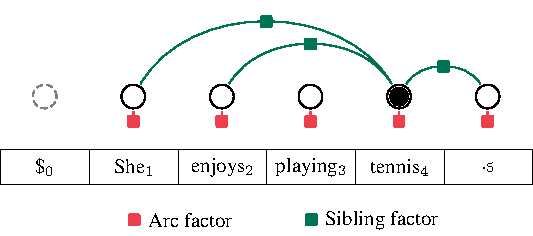
\includegraphics[scale=1]{figures/dep-factors.pdf}
		\caption{依存句法模型的因子图}
		\label{fig:dep-factors}
	\end{subfigure}
	\begin{subfigure}[b]{0.8\textwidth}
		\centering
		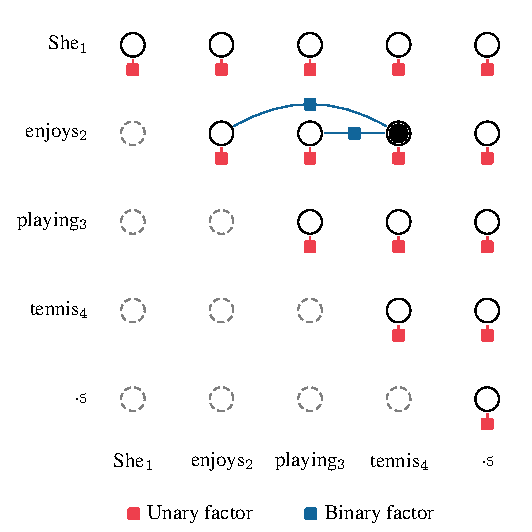
\includegraphics[scale=1]{figures/con-factors.pdf}
		\caption{成分句法模型的因子图}
		\label{fig:con-factors}
	\end{subfigure}
	\caption{一个例句和其依存/成分句法模型对应的因子图,我们在例句上方标出了对应的正确无标签依存句法树和成分句法树,其中成分句法树进行了左二叉化.
		灰色虚线圆圈代表被屏蔽的变量.
		图中标出了所有的一阶(红色)因子,为了简洁起见,对于二阶因子,依存句法图中我们只标出了涉及弧$3\rightarrow 4$的兄弟(绿色)因子,成分句法图中只标出了和组块$(3, 4)$连接的二阶(蓝色)因子.}
	\label{fig:vi-factors}
\end{figure}

目前广泛使用的一阶局部模型(对应于章节~\ref{cha:dep-crf}的\textsc{Loc}方法,这里我们称为\textsc{Loc}$_{dep}$)在训练的时候采用了头选择(head selection)的训练损失函数,要求句子中除了根结点之外的每个词有且仅有一个头.
和\citet{wang-tu-2020-second}一样,我们选择在依存句法对应变分推断方法中引入头选择约束,相应的因子图设计见图~\ref{fig:dep-factors}.
对于每个位置$j$,我们定义变量取值$y_j\in \{0,1,\cdots,i\neq j,\cdots,n\}$,代表词$w_j$的可能的头索引.

具体地,对于每个变量$y_j$,一阶的势函数定义为
\begin{equation}
	\label{eq:dep-1o-potential}
	\psi_j(y_j)=\exp(\mathrm{s}(y_j\rightarrow j))
\end{equation}
$\mathrm{s}(y_j\rightarrow j)$是弧$y_j\rightarrow j$对应的分值,由公式~\ref{eq:biaffine}计算得到.

对于包含两个变量$y_{j}$和$y_{k}$的二阶因子,对应的势函数定义为
\begin{equation}
	\label{eq:2o-dep-potential}
	\psi_{j,k}(y_j,y_k)=\left\{
	\begin{array}{rcl}
		\exp \mathrm{s}(y_j\rightarrow \{k,j\}) &   & {y_j=y_k}   \\
		1                                       &   & {otherwise}
	\end{array}
	\right.
\end{equation}
$\mathrm{s}(y_j\rightarrow \{k,j\})$是兄弟子树$y_j\rightarrow \{k,j\}$的分值,由公式~\ref{eq:triaffine}计算得到.
需要注意的是这里的兄弟$k$和二阶TreeCRF不同,并不需要一定和$j$邻近 \citep{smith-eisner-2008-dependency}.
我们要求子树$y_j\rightarrow \{k,j\}$中没有环存在,即有$k\neq {0,j,y_j}$.

MFVI迭代式地更新近似分布$Q(\cdot)$,来最小化其与真实分布$P(\cdot)$的KL散度.
依存句法模型的迭代更新公式如下 \citep{wang-tu-2020-second}:
\begin{equation}
	\label{eq:mfvi-dep}
	Q_{j}^{(t)}(i)\propto \exp\left(\mathrm{s}(i\rightarrow j) +\sum_{k\neq i,j} Q_{k}^{(t-1)}(i)\cdot \mathrm{s}(i\rightarrow {k,j}) \right)
\end{equation}
后验分布$Q_j^{(0)}(i)$初始化为一阶势函数的值$\psi_j(i)$.
每次迭代时,我们都会将$Q_j^{(t)}(\cdot)$的值在所有可能的头取值上进行归一化.
经过$T$次迭代后,我们得到最终的近似后验分布$Q_j^{(T)}(\cdot)$.

\subsection{成分句法的MFVI方法}\label{sec:con-vi}

我们的成分句法分析模型采用了\citet{gaddy-etal-2018-whats}的方法作为基线方法,称为\textsc{Loc}$_{con}$.
具体来说,模型对短语树所有可能的位置进行一个简单的二分类,预测该位置是否是一个区块.
\citet{dozat-manning-2018-simpler,wang-etal-2019-second}在语义依存分析中应用了这样的训练目标.
\citet{gormley-eisner-2015-structured,naradowsky-etal-2012-grammarless}在成分句法分析中应用了这种方法.
我们将其引入到了基于MFVI的成分句法分析中,并采用了一个一阶因子和一个二阶因子,对应的因子图见图~\ref{fig:con-factors}.

具体地,每个位置$ij$的可能的变量取值$y_{ij}\in \{0,1\}$.
其中单个变量$y_{ij}$的一阶的势函数定义为
\begin{equation}
	\label{eq:con-1o-potential}
	\psi_{ij}(y_{ij})=\left\{
	\begin{array}{rcl}
		\exp\left(\mathrm{s}(i,j)\right) &   & {y_{ij}=1}  \\
		1                                &   & {otherwise}
	\end{array}
	\right.
\end{equation}
$\mathrm{s}(i,j)$是由公式~\ref{eq:con-biaffine}计算得到的区块$(i,j)$的分值,这里我们要求$i<j$.

给定两个变量$y_{ij}$和$y_{lk}$,我们使用章节~\ref{cha:con-crf}的二阶兄弟特征,因此二阶的势函数定义为
\begin{equation}
	\label{eq:2o-con-potential}
	\psi_{ij,lk}(y_{ij},y_{lk})=\left\{
	\begin{array}{rcl}
		\exp\left(\mathrm{s}(i,k,j)\right) &   & {i=l}       \\
		1                                  &   & {otherwise}
	\end{array}
	\right.
\end{equation}
$\mathrm{s}(i,k,j)$可以视为$(i,j)$和$(i,k)$都作为组块时,组成的子树的分值,由公式~\ref{eq:con-triaffine}计算得到.
需要注意的是这里$k$的位置不受动态规划算法的约束,并不要求一定位于$(i,j)$之间,即有$i<k,k\neq j$.

成分句法模型的MFVI迭代更新公式如下:
\begin{equation}
	\label{eq:mfvi-con}
	\begin{array}{l}
		Q_{ij}^{(t)}(0)\propto 1                                                                                            \\
		Q_{ij}^{(t)}(1)\propto \exp\left(\mathrm{s}(i,j) +\sum_{k\neq i,j} Q_{ik}^{(t-1)}(1)\cdot \mathrm{s}(i,k,j) \right)
	\end{array}
\end{equation}
后验概率$Q_{ij}^{(0)}(y_{ij})$初始化为一阶势函数$\psi_{ij}(y_{ij})$.
每次迭代时,我们将$Q_{ij}^{(t)}(\cdot)$在取值$\{0,1\}$上进行归一化.
经过$T$次迭代后,我们得到成分句法最终的近似后验分布$Q_{ij}^{(T)}(\cdot)$.

\subsection{训练损失函数}

我们的训练损失函数分为两部分,分别是无标签树的损失和对应标签的损失.
给定所有正确标签,我们的目标是最大化树上每个标签的概率,和前面的章节一致,我们采用了弧/区块级别的标准交叉熵损失函数.
给定输入句子$\boldsymbol{x}$和对应正确的无标签句法树$\boldsymbol{y}^{\ast}$,我们的目标是最大化句法树的概率$p(\boldsymbol{y}^{\ast}\mid\boldsymbol{x})$.
由于MFVI将真实分布在每个变量上分解得到近似概率分布$Q(\cdot)$,因此训练目标等价于最大化每个变量的后验概率.

其中,对于每个句子,依存句法分析树采用了弧分解策略,每个位置的变量取值为所有可能的头,因此相应无标签句法树的损失函数为
\begin{equation}
	\label{eq:dep-vi-arc-loss}
	L_{dep}^{tree}=-\sum_{j\neq 0}\log Q_j(y^{\ast}_j)
\end{equation}

成分句法的无标签句法树按照组块分解,每个组块可能的取值为$\{0,1\}$,因此目标函数为
\begin{equation}
	\label{eq:con-vi-bracket-loss}
	L_{con}^{tree}=-\sum_{i<j}\log Q_{ij}(y^{\ast}_{ij})
\end{equation}
参考\citet{dozat-manning-2018-simpler},我们还新引入了一个参数$\lambda$用于平衡无标签句法树以及标签的损失,相应的成分句法的最终训练目标为
\begin{equation}
	\label{eq:con-vi-loss}
	L_{con}=\lambda L_{con}^{label}+(1-\lambda)L_{con}^{tree}
\end{equation}

\subsection{解码}
我们在MFVI模型中解码时直接应用了MBR解码的策略.
我们采用MFVI近似得到的后验概率$Q(\cdot)$代替边缘概率作为解码算法的输入.
依存句法中,我们将由公式~\ref{eq:mfvi-dep}得到的概率$Q_i(\cdot)$作为输入,并利用了Eisner算法来解码,加速时采用了算法~\ref{alg:eisner-2o}的批次化技术.
成分句法中,我们将由公式~\ref{eq:mfvi-con}得到的概率$Q_{ij}(\cdot)$作为输入,并利用了和章节~\ref{cha:con-crf}一样的类CKY算法来解码,采用了算法~\ref{alg:inside}的批次化技术来加速.

\section{实验}\label{sec:vi-exp}

\noindent\textbf{参数设置.}
我们保持两种句法分析模型的编码器和训练方法与前面的章节基本一致.
对于二阶模型,我们设置依存句法分析中使用的兄弟特征以及成分句法分析使用的二阶特征的MLP层输出维度为100.
我们设置变分推断的迭代次数统一为3次.
对于在成分句法分析中的用于平衡标签和无标签树的训练损失的参数$\lambda$,我们设置为0.1.

\noindent\textbf{模型定义.}
我们在每种句法分析上都比较了四种模型:\textsc{Loc}、\textsc{Crf}、\textsc{Crf2o}和\textsc{Mfvi},这里有必要对于他们的记号做一下说明.
\textsc{Loc}表示采用了局部损失函数的模型,\textsc{Crf}和\textsc{Crf2o}指的是使用了一阶和二阶精确推断的TreeCRF模型,\textsc{Mfvi}表示采用平均场变分推断的模型.
相同记号的在各自任务的指导不同,例如依存模型中的\textsc{Loc}采用了头选择损失函数,而成分模型的\textsc{Loc}采用了二分类损失函数.
有时候我们会附加下标$dep$和$con$以示区分.

\begin{table}[tb!]
  \centering
  \caption{依存句法分析模型在PTB和CoNLL09的Test数据上不同推断算法的结果.}
  \begin{tabular}{lcccc}
    \toprule
                   & \multicolumn{2}{c}{PTB} & \multicolumn{2}{c}{CoNLL09}                                   \\
                   & UAS                     & LAS                         & UAS            & LAS            \\[2pt]
    \midrule
    \\[-15pt]
    \textsc{Loc}   & 96.08                   & 94.47                       & 89.15          & 85.98          \\
    \textsc{Crf}   & 96.02                   & 94.33                       & 89.28          & 86.18          \\
    \textsc{Mfvi}  & \textbf{96.11}          & \textbf{94.49}              & 89.35          & 86.25          \\
    \textsc{Crf2o} & \textbf{96.11}          & 94.46                       & \textbf{89.63} & \textbf{86.52} \\
    \multicolumn{5}{c}{+BERT}                                                                                \\[3pt]
    \textsc{Loc}   &                                                                                         \\
    \textsc{Crf}   &                                                                                         \\
    \textsc{Mfvi}  &                                                                                         \\
    \textsc{Crf2o} &                                                                                         \\
    \bottomrule
  \end{tabular}
  \label{table:vi-dep-test}
\end{table}




\subsection{主要结果}
表格~\ref{table:vi-dep-test}和表格~\ref{table:vi-con-test}分别给出了我们尝试的多种推断算法在依存句法和成分句法分析上的比较性实验结果.
和章节~\ref{cha:dep-crf}以及章节~\ref{cha:con-crf}一样,我们在所有模型中都使用了预训练词向量作为输入.
英文数据我们统一使用了100维的Glove词向量,中文数据则使用了word2vec在Giga数据上训练的100维词向量.
我们还汇报了BERT的结果,对于英文数据,我们使用了24层1024维的\texttt{bert-large-cased}作为双向LSTM的输入,并在训练时固定参数.
中文数据我们则使用了12层768维的\texttt{bert-base-chinese}.

可以看到在依存句法的结果上(表格~\ref{table:vi-dep-test}),由于英文PTB的结果非常高,因此这四种推断方法的结果都十分接近,\textsc{Mfvi}方法超越了\textsc{Loc},达到了最好的性能.
中文CoNLL09上,精确推断的\textsc{Crf2o}仍然是最好的,但是\textsc{Mfvi}超越了\textsc{Crf}达到了86.25的LAS.
在两种语言上,\textsc{Mfvi}都一致超越了没有全局结构约束的\textsc{Loc}方法.
这验证了在近似推断的\textsc{Mfvi}方法上应用二阶结构约束的有效性.

在成分句法分析上(表格~\ref{table:vi-con-test}),中英文三个数据的结果中,无论是一阶\textsc{Crf}还是二阶\textsc{Crf2o},精确推断算法都仍然是表现最好的.
然而\textsc{Mfvi}都达到了和一阶\textsc{Crf}十分相近的性能.
并且,\textsc{Mfvi}一致超越了基于二分类学习的\textsc{Loc}模型,在PTB、CTB51和CTB7上分别提升了0.11、0.52和0.35.

当使用BERT之后,上述的几种推断算法在结果上没有显著差异.
依存句法上,PTB中\textsc{Mfvi}表现最好,LAS为95.37,达到或超越了当前的最佳性能 \citep{zhou-zhao-2019-head,wang-tu-2020-second},CoNLL09上仍然\textsc{Crf2o}最佳,但是\textsc{Mfvi}的差距十分微弱.
成分句法中在PTB和CTB51这两个数据上,\textsc{Mfvi}的表现都是最好的,分别达到95.71和92.56的$\mathrm{F}_1$值,高于当前最佳的模型\citep{kitaev-etal-2019-multilingual}.
在CTB7上表现最好的仍是\textsc{Crf2o},$\mathrm{F}_1$值为91.62,而\textsc{Mfvi}的差距不到0.1.
然而,基于\textsc{Mfvi}方法的近似推断在解析效率上有很大的优越性(见章节~\ref{sub@sec:vi-speed}的复杂度分析).

\begin{table}[tb!]
  \centering
  \caption{成分句法分析模型在英文PTB、中文CTB5.1和CTB7的Test数据上不同推断算法的结果.}
  \begin{tabular}{lccccccccc}
    \toprule
                   & \multicolumn{3}{c}{PTB} & \multicolumn{3}{c}{CTB51} & \multicolumn{3}{c}{CTB7}                                                                                                       \\
                   & $\mathrm{P}$            & $\mathrm{R}$              & $\mathrm{F}_1$           & $\mathrm{P}$   & $\mathrm{R}$   & $\mathrm{F}_1$ & $\mathrm{P}$   & $\mathrm{R}$   & $\mathrm{F}_1$ \\[2pt]
    \midrule
    \\[-15pt]
    \textsc{Loc}   & 94.16                   & 93.85                     & 94.01                    & 89.39          & 89.16          & 89.28          & 88.54          & 87.96          & 88.25          \\
    \textsc{Crf}   & 94.23                   & 94.02                     & 94.12                    & 89.71          & \textbf{89.89} & 89.80          & 88.84          & 88.36          & 88.60          \\
    \textsc{Mfvi}  & 94.11                   & 93.96                     & 94.04                    & 89.82          & 89.79          & \textbf{89.81} & 88.71          & 88.16          & 88.43          \\
    \textsc{Crf2o} & \textbf{94.29}          & \textbf{94.15}            & \textbf{94.22}           & \textbf{89.97} & 89.47          & 89.72          & \textbf{88.95} & \textbf{88.56} & \textbf{88.76} \\
    \multicolumn{10}{c}{+BERT}                                                                                                                                                                            \\[3pt]
    \textsc{Loc}   & 95.70                   & 95.43                     & 95.57                    & 92.47          & 92.09          & 92.28          & 91.90          & 91.24          & 91.57          \\
    \textsc{Crf}   & 95.85                   & 95.53                     & 95.69                    & 92.51          & 92.04          & 92.27          & 91.73          & \textbf{91.38} & 91.55          \\
    \textsc{Mfvi}  & 95.85                   & \textbf{95.57}            & \textbf{95.71}           & \textbf{92.78} & \textbf{92.35} & \textbf{92.56} & 91.89          & 91.31          & 91.60          \\
    \textsc{Crf2o} & \textbf{95.86}          & 95.47                     & 95.67                    & 92.75          & 92.18          & 92.47          & \textbf{91.93} & 91.31          & \textbf{91.62} \\
    \bottomrule
  \end{tabular}
  \label{table:vi-con-test}
\end{table}




\subsection{样例分析}

\begin{figure}[tb!]
	\centering
	\begin{subfigure}[b]{0.9\textwidth}
		\centering
		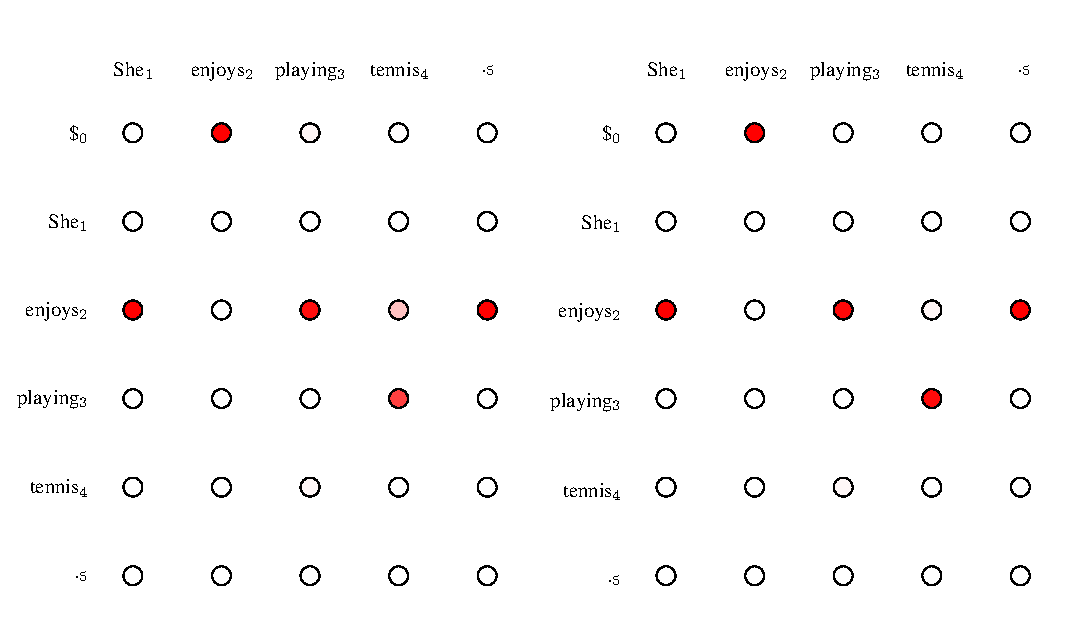
\includegraphics[scale=0.75]{figures/dep-probs.pdf}
		\caption{依存句法树每个位置对应的分值和后验概率}
		\label{fig:dep-probs}
	\end{subfigure}
	\begin{subfigure}[b]{0.9\textwidth}
		\centering
		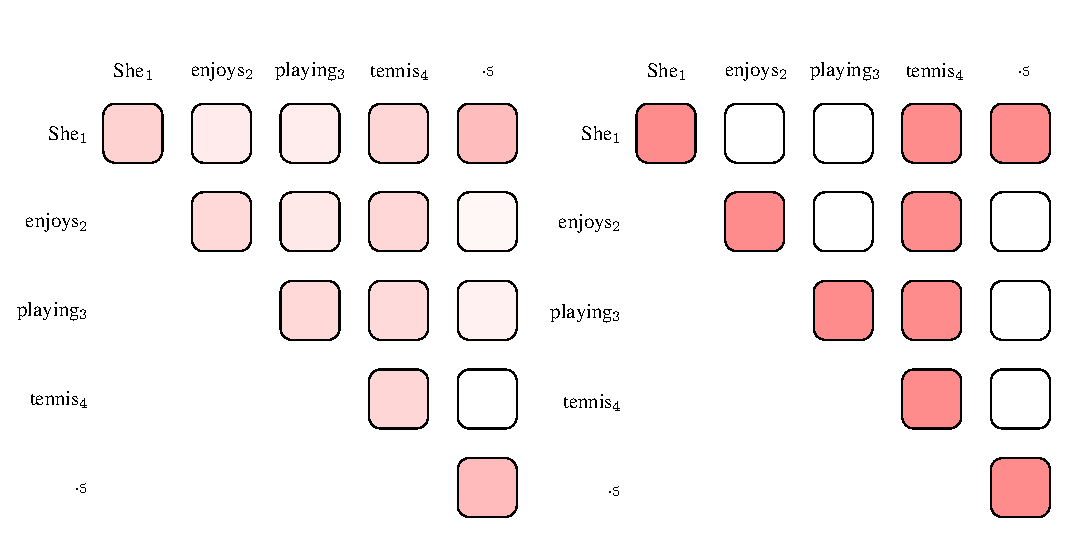
\includegraphics[scale=0.75]{figures/con-probs.pdf}
		\caption{成分句法树每个位置对应的分值和后验概率}
		\label{fig:con-probs}
	\end{subfigure}
	\caption{一个例句对应的依存句法模型和成分句法模型的输出.
		左边的图是每个位置的分值(log potential),为了方便显示,我们首先对分值进行了归一化.
		右边的图是变分推断得到的后验概率.
	灰色虚线圆圈代表被屏蔽的不合法位置.}

	\label{fig:vi-probs}
\end{figure}

图~\ref{fig:vi-probs}给出了一个例句分别在依存和成分句法模型上的分值(log potentials)与经过MFVI迭代近似得到的后验概率的热力图对比.
图中颜色的深浅反应了分值/概率的大小.

左边的图反应的是模型直接输出的分值之间的对比,这对应于一阶模型的输出.
可以看到模型的输出的分值数值相对来说都比较均匀.
由于依存句法模型基于的是头选择的训练目标,可以看到图中的每一列都有一个极值存在,比如词$She_i$对应的列中,颜色最深(分值最高)的位置为词$enjoys_2$,这对应了句法树中的弧$enjoys_2\rightarrow She_1$.
成分句法的热力图中,由于采用了二分类的目标,因此颜色较深的位置表示更可能成为一个区块.
然而由于没有类似于依存句法的头约束,直接通过对每个位置$\arg\max$得到的所有区块可能无法组成一棵合法的句法树,因此我们仍需要CKY算法来获得全局最优的合法句法树.

当我们利用MFVI算法,得到的近似后验概率的热力图如右边图所示.
可以看到,在进一步考虑了二阶特征的分值并聚合到每个变量位置之后,后验概率的置信度远远高于分值.
对于依存句法而言,每个词都有一个最可能的头,并且概率几乎为1,对应于热力图中每列仅有一个红色结点.
对于成分句法而言,如果对图中每个位置的后验概率取$\arg\max$得到可能的区块,每个区块的概率同样近似为1,并且对于图中的例句而言,这种贪婪解码得到的句法树可以直接组成一棵合法的短语结构树,例如,红色结点$(She_1,tennis_4)$和$(playing_3,tennis_4)$对应了例句正确的无标签树左二叉化之后的两个区块.
这显示了MFVI在引入二阶结构打分之后,对于模型结构预测更强大的约束作用.


\subsection{速度和时间复杂度比较}
\label{sub@sec:vi-speed}
\begin{table}[tb!]
  \centering
  \caption{依存句法和成分句法使用不同推断算法的时间复杂度,以及相应的在PTB的Test数据上的解析时间的比较.
    依存句法统一使用了Eisner算法解码,成分句法统一使用了CKY算法解码}
  \begin{tabular}{llcccr}
    \toprule
     & \multirow{2}{*}{Inference} & \multicolumn{2}{c}{Complexity} & \multirow{2}{*}{Decoding Alg.} & \multirow{2}{*}{Sents/sec}                 \\
     &                            & CPU                            & GPU                            &                            &               \\[2pt]
    \midrule
    \multirow{3}{*}{Dependency}
    % & \textsc{Loc}               & $O(n)$                         & $O(1)$                         & Eisner                     & 990           \\
     & \textsc{Crf}               & $O(n^3)$                       & $O(n^2)$                       & Eisner                     & 653           \\
     & \textsc{Crf2o}             & $O(n^3)$                       & $O(n^2)$                       & Eisner                     & 431           \\
     & \textsc{Mfvi}              & $O(n^3)$                       & $O(n)$                         & Eisner                     & \textbf{1126} \\
    \midrule
    \multirow{3}{*}{Constituency}
    % & \textsc{Loc}               & $O(n)$                         & $O(1)$                         & CKY                        & 990           \\
     & \textsc{Crf}               & $O(n^3)$                       & $O(n^2)$                       & CKY                        & 743           \\
     & \textsc{Crf2o}             & $O(n^3)$                       & $O(n^2)$                       & CKY                        & 598           \\
     & \textsc{Mfvi}              & $O(n^3)$                       & $O(n)$                         & CKY                        & \textbf{905}  \\

    \bottomrule
  \end{tabular}
  \label{table:vi-speed}
\end{table}
表~\ref{table:vi-speed}给出了\textsc{Mfvi}和前面章节提及的精确推断模型的速度和复杂度的比较.
为了统一比较,所有的设置下都应用了MBR解码,并且每个任务都用了相同的解码算法.
可以看到,无论是依存句法还是成分句法模型,他们相应的\textsc{Mfvi}在CPU上每一次迭代都需要$O(n^3)$的复杂度,这和精确推断的2阶Inside算法的复杂度相当.
而当利用GPU进行并行计算时,\textsc{Mfvi}每个位置的变量仅需要一次遍历来收集其他位置的信息\footnote{尽管现代的CUDA技术可以通过二叉树等数据结构让并行化的归约操作,例如$\mathrm{sum}$、$\mathrm{min}$和$\mathrm{max}$等,缩减到$O(\log n)$复杂度的时间 \citep{wang-etal-2020-ain},但是这里我们统一假设归约操作的复杂度为$O(n)$.},因此GPU上的算法复杂度为$O(n)$,大大快于精确推断所需要的$O(n^2)$复杂度.

从表中可以看到,利用\textsc{Mfvi}的依存句法在PTB的Test数据的解析速度为1126句每秒,是精确推断的二阶\textsc{Crf2o}(431)的近三倍快,同样也大大快于一阶\textsc{Crf}的557句每秒.
成分句法的\textsc{Mfvi}模型的解析速度大约为905句每秒,同样显著快于一阶\textsc{Crf}的743句每秒和二阶\textsc{Crf2o}的598句每秒.

\section{本章小结}

在本章我们将包含高阶特征的MFVI方法方法引入到了依存句法和成分句法分析中,以解决精确推断的高阶方法的高复杂度问题.
根据两种句法分析的特点,在依存句法分析上,我们实现了一个包含头选择约束的MFVI方法,在成分句法分析上,我们引入了一个基于二分类学习目标的MFVI方法.
在这两个句法任务的中英文个五个数据集上的结果表明,MFVI方法均显著超越了基于局部学习的一阶方法,并达到和精确推断的二阶TreeCRF方法可比较的性能.
在速度上,我们的MFVI方法分别在依存和成分句法达到了1126句每秒和905句每秒的解析速度.
加入BERT之后,基于MFVI方法的近似推断模型在所有的数据集上都达到或者接近了当前最佳模型的性能.
